\documentclass[a4paper, 12pt]{article}
\usepackage[top=2cm, bottom=2cm, left=2.5cm, right=2.5cm]{geometry}
\usepackage[utf8]{inputenc}
\usepackage[brazilian]{babel}
\usepackage{indentfirst}
\usepackage{graphicx}
\usepackage{wrapfig}
\usepackage[pdftex]{hyperref}
\graphicspath{ {imagens/} }
\usepackage{amsmath}

\begin{document}
%
\begin{titlepage} %iniciando a "capa"
	\begin{center} %centralizar o texto abaixo
		{\large Unicamp}\\[0.4cm] %0,2cm é a distância entre o texto dessa linha e o texto da próxima
		{\large Marco Lucio Bittencourt - Turma B}\\
		{\large Heitor Nigro Lopes - PED}\\[3.2cm]
		{\bf \huge Dinâmica Trabalho 2}\\[0.2cm] 
		{\bf \large Matrizes de Rotação e Range Kutta}\\[4.9cm]
		% o comando \bf deixa o texto entre chaves em negrito. O comando \huge deixa o texto enorme
	\end{center} %término do comando centralizar
	{\large Erik Yuji Goto}\\ % o comando \large deixa o texto grande
	RA: 234009\\[10cm]
	\begin{center}
	
		{\large Campinas}\\[0.2cm]
		{\large 2021}
	\end{center}
\end{titlepage} %término da "capa"


\tableofcontents
\newpage

\section{Passo a passo para resolver as questões}
	\begin{enumerate}
	\item Escolher eixos coordenados
	\item Diagrama de corpo livre
	\item Aplicar Lei de Newton
	\item Resovler a EDO
	\end{enumerate}		
	
\section{1 grau de liberdade}
\subsection{Vibrações livres não amortecidas de 1 grau de liberdade(DOF)}
	
	\begin{figure}[h]
	\centering
	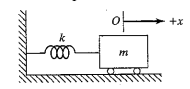
\includegraphics[scale=1.5]{a.png}
	\caption{1 DOF não amortecido}
	\end{figure}
	
	A solução é dada por:
	
	\begin{equation}
	\boxed{X(t) = A sin(\omega_n t + \phi)}
	\end{equation}
	
	Onde,
	
	\begin{equation}
	\boxed{\omega_n = \sqrt{\frac{k}{m}}}
	\end{equation}

	Para condições iniciais nulas, $X_0 = X(0)$ e $V_0 = \dot{X}(0)$ as constantes são:
	\begin{equation}
	\boxed{\phi = tg^{-1} \frac{\omega_n X_0}{V_0}}
	\end{equation}
	\begin{equation}
	\boxed{A = \frac{\sqrt{\omega_n^2 X_0^2 + V_0^2}}{\omega_n}}
	\end{equation}

	Para um \textit{sistema massa-mola na vertical}, o peso \textbf{mg} é equilibrado por uma distenção inial da mola. O bloco oscila ao redor do \textbf{ponto de equilíbrio estático}.

\subsection{Molas Equivalentes}
\newpage
\subsubsection{Viga Engastada}
	\begin{figure}[h]
	\centering
	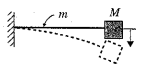
\includegraphics[scale=1.5]{a1.png}
	\caption{Viga Engastada}
	\end{figure}
	
	\begin{equation}
	K = \frac{3EI}{l^3}
	\end{equation}
	E = módulo de elasticidade\\
	I = momento de inércia
	
\subsubsection{Viga Biapoiada}
	\begin{figure}[h]
	\centering
	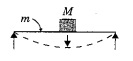
\includegraphics[scale=1.5]{a2.png}
	\caption{Viga Biapoiada}
	\end{figure}
	
	\begin{equation}
	K = \frac{48EI}{l^3}
	\end{equation}

\subsubsection{Barra em Solicitação Axial}
	\begin{figure}[h]
	\centering
	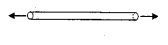
\includegraphics[scale=1.5]{a3.png}
	\caption{Barra em Solicitação Axial}
	\end{figure}
	
	\begin{equation}
	K = \frac{AE}{l}
	\end{equation}	
	A = Área transversal
	
\newpage
\subsubsection{Molas em Paralelo}
	\begin{figure}[h]
	\centering
	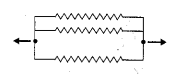
\includegraphics[scale=1.5]{a4.png}
	\caption{Molas em Paralelo}
	\end{figure}
	
	\begin{equation}
	K_{eq} = \sum^n_{i =1} K_i
	\end{equation}
	$\Delta$ é igual para todas as molas
	
\subsubsection{Molas em Série}
	\begin{figure}[h]
	\centering
	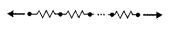
\includegraphics[scale=1.5]{a5.png}
	\caption{Molas em Série}
	\end{figure}
	
	\begin{equation}
	K_{eq} = (\sum^n_{i = 1}\frac{1}{K_i})^{-1}
	\end{equation}
	A força é igual para todas as molas
	

\subsection{Sistema Torcional}
	\begin{figure}[h]
	\centering
	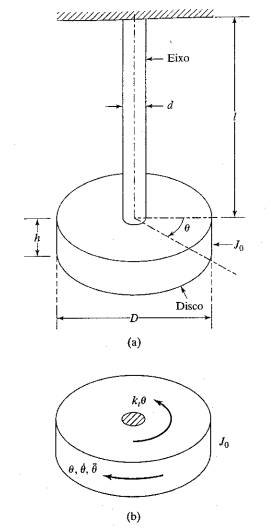
\includegraphics[scale=0.5]{a6.png}
	\caption{Sistema Torcional}
	\end{figure}
	
	\begin{equation}
	J\ddot{\theta} = -K_t \theta
	\end{equation}
	\begin{equation}
	\boxed{\ddot{\theta} + \frac{K_t}{J}\theta = 0}
	\end{equation}
	Neste caso, $\omega_n^2 = \frac{K_t}{J}$
	
\subsection{Vibrações Livres de Sistema de 1 GDL amortecidas}
	
	[imagem]\\
	
	Equação do sistema:
	\begin{equation}
	\boxed{\ddot{x} + \frac{c}{m}\dot{x}+\frac{K}{m}x = 0}
	\end{equation}
	
	O valor da constante de amortecimento tal que $\frac{Cc}{2m} = \sqrt{\frac{K}{m}} = \omega_n$ é chamado de \textbf{amortecimento crítico}.
	
	Ou ainda,
	\begin{equation}
	\boxed{C_c = 2m\omega_n = 2\sqrt{mK}}
	\end{equation}
	
	Seja $\boxed{\xi =\frac{C}{C_c}}$ o \textbf{fator de amortecimento} (adimensional). Verifica-se que: $\frac{c}{2m} = \xi \omega_n$, logo
	\begin{equation}
	\boxed{\ddot{x} + 2 \xi \omega_n \dot{x} + \omega_n^2x = 0 \ (forma\ padronizada)}
	\end{equation}
	
	A \textbf{frequência natural amorteciad} é dada por:
	\begin{equation}
	\boxed{\omega_d = \omega_n \sqrt{1-\xi^2}}
	\end{equation}
	
\subsubsection{Amortecimento Subcrítico(subamortecido)}
	$\xi < 1$\\
	\begin{equation}
	\boxed{x(t) = Xe^{-\xi \omega_n t}sin(\omega_d t + \phi)}
	\end{equation}
	
	Através das condições iniciais determinam-se X e $\phi$
	
\subsubsection{Amortecimento Crítico}
	$\xi = 1$ ; $s_1 = s_2 = -\xi \omega_n = -\omega_n$
	\begin{equation}
	\boxed{x(t) = A_1 e^{-\omega_n t} + A_2 t e^{-\omega_n t}}
	\end{equation}
	Note que, não há oscilação
	
\subsubsection{Amortecimento Supercrítico(superamortecido)}
	$\xi > 1$ ; $s_1 = \omega_n (\xi + \sqrt{\xi^2 - 1}) = \frac{-1}{\delta_1}$ ; $s_1 = \omega_n (-\xi - \sqrt{\xi^2 - 1}) = \frac{-1}{\delta_2}$

	\begin{equation}
	\boxed{x(t) = A_1 e^{\frac{-t}{\delta_1}} + A_2 e^{\frac{-t}{\delta_2}}}
	\end{equation}
	
\subsection{Decremento Logarítimico}
	Para n períodos:
	\begin{equation}
	\boxed{\delta = \xi \omega_n T = \frac{1}{n} ln\frac{x(t)}{x(t + nT)}}
	\end{equation}
	
	\begin{equation}
	\boxed{\xi = \frac{\delta}{\sqrt{4 \pi^2 + \delta^2}}}
	\end{equation}
	
\subsection{Amortecimento de Coulomb}
	
	[to do it]
	
\subsection{Vibrações forçadas - 1 DOF não amortecido (excitação harmônica)}
	[imagem]\\
	
	Equação do movimento:
	\begin{equation}
	\ddot{x} + \frac{K}{m}x = \frac{F_0}{m}cos(\Omega t) = f_0 cos(\Omega t)
	\end{equation}

	Solução Homogênea
	\begin{equation}
	x_h = A_1 sin(\omega_n t) + A_2 cos(\omega_n t)
	\end{equation}
	
	Solição Particular
	\begin{equation}
	x_p = X cos(\Omega t)
	\end{equation}
	
	Substituindo $x_p$ na eq. diferencial, encontramos o valor de X:
	\begin{equation}
	X = \frac{f_0}{\omega_n^2 - \Omega} \ para \ \omega_n \neq \Omega
	\end{equation}
	
	Solução completa:
	\begin{equation}
	\boxed{x(t) = A_1 sin(\omega_n t) + A_2 cos(\omega_n t) + \frac{f_0}{\omega_n^2 - \Omega^2} cos(\Omega t)}
	\end{equation}
	
	Usando como condições iniciais $x(0) = \dot{x}(0) = 0$, logo
	\begin{equation}
	x(t) = \frac{2f_0}{\omega_n^2 - \Omega^2} sin(\frac{\omega_n - \Omega t}{2}) sin(\frac{\omega_n + \Omega}{2} t)
	\end{equation}
	
\newpage
	Como $\Omega \Delta$, a curva $sin(\Omega t)$ será modulada pela curva $sin(\Delta t)$
	\begin{figure}[h]
	\centering
	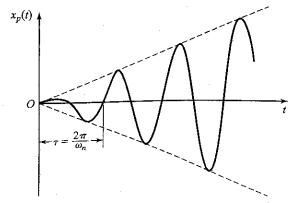
\includegraphics[scale=0.8]{a7.png}
	\caption{Batimento}
	\end{figure}
	
	Quando $\Omega \rightarrow \omega_n \Rightarrow \Delta t \rightarrow 0 \Rightarrow sin(\Delta t) \cong \Delta t$ 
	\begin{equation}
	x(t) = \frac{f_0}{2\Omega} t sin(\Omega t)
	\end{equation}
	
	\begin{figure}[h]
	\centering
	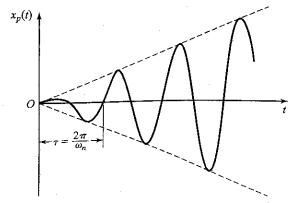
\includegraphics[scale=0.8]{a7.png}
	\caption{Ressonância}
	\end{figure}
	
\subsection{Vibrações forçadas - 1 DOF amortecimento viscoso (excitação harmônica)}
	A equação de movimento é dada por:
	\begin{equation}
	m\ddot{x} + c \dot{x} + Kx = F_0 sin(\Omega t)
	\end{equation}
	\begin{equation}
	\ddot{x} + \frac{c}{m}\dot{x} + \frac{K}{m}x = \frac{F_0}{m} sin(\Omega t)
	\end{equation}
	\begin{equation}
	\ddot{x} + 2 \xi \omega_n \dot{x} + \omega_n^2 x = f_0 sin(\Omega t)
	\end{equation}
	
	Solução Homgênea:
	\begin{equation}
	x_n(t) = A e^{-\xi \omega_n t} sin(\omega_d t + \phi)
	\end{equation}
	Solução Particular:
	\begin{equation}
	x_p(t) = M sin(\Omega t) + N cos(\Omega t)
	\end{equation}
	
	\begin{equation}
	\boxed{r = \frac{\Omega}{\omega_n}  \ (razao \ de\ frequencia)}
	\end{equation}
	
	Derivando $x_p$ e substituindo na equação do movimento conseguimos encontrar \textbf{M} e \textbf{N}:
	\begin{equation}
	\boxed{M = \frac{(1 - r^2)\frac{f_c}{\omega_n^2}}{(1-r^2)^2 + (2\xi r)^2}}
	\end{equation}
	\begin{equation}
	\boxed{N = \frac{-2 \xi \frac{f_0}{\omega_n^2}}{(1-r^2)^2 + (2\xi r)^2}}
	\end{equation}
	
	No livro do Boyce temos a seguinte relação para a solução particular:
	\begin{equation}
	x_p(t) = X sin(\Omega t - \Theta)
	\end{equation}
	Onde,
	\begin{equation}
	X = \sqrt{M^2 + N^2} = \frac{f_0/\omega_n^2}{\sqrt{(1-r^2)^2 + (2 \xi r)^2}}
	\end{equation}
	
	Definimos \textbf{fator de amplificação} como:
	\begin{equation}
	MF =  \frac{XK}{F_0} = \frac{X \omega_n^2}{f_0} = \frac{1}{\sqrt{(1-r^2)^2 + (2\xi r)^2}}
	\end{equation}
	
	
	\begin{figure}[h]
	\centering
	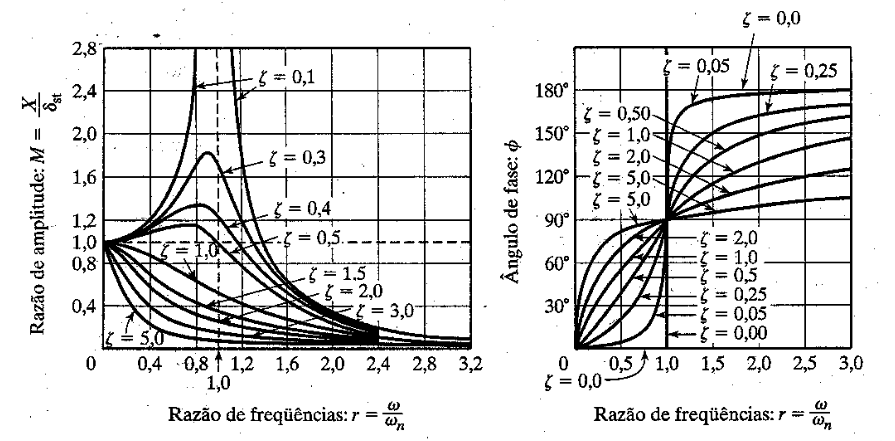
\includegraphics[scale=0.7]{a9.png}
	\caption{Relações de r x MF e r x $\phi$}
	\end{figure}
\newpage
	Pela figura concluímos que:
	\begin{enumerate}
	\item Para um sistema não amortecido ($\xi = 0$), $M\rightarrow \infty$ quando $r\rightarrow 1$
	\item Qualquer quantidade de amortecimento reduz o fator de amplificação
	\item $M\rightarrow 0$ quando $r\rightarrow \infty$
	\item Para $0 < \xi< \frac{1}{\sqrt{2}}$, o valor máximo de M ocorre quando
		\begin{equation}
		r= \sqrt{1-2\xi^2} \ ou\ \omega = \omega_n\sqrt{1- 2 \xi^2}
		\end{equation}
	\item Quando $r= \sqrt{1-2\xi^2}$ o valor máximo de M é
		\begin{equation}
		M_{max} = \frac{1}{2\xi \sqrt{1- \xi^2}}
		\end{equation}
	\end{enumerate}		
	
\subsection{Desbalanceamento Rotativo}
	[imagem]
	\begin{equation}
	M\ddot{x} + c \dot{x} + Kx = m e \Omega^2 sin(\Omega t)
	\end{equation}
	
	Solução particular(lembrando que a solução homogênea desaparece no regime permanente):
	\begin{equation}
	x_p(x) = X sin(\Omega t - \theta)
	\end{equation}
	
	\begin{equation}
	\boxed{X = \frac{(me\Omega^2/M)/\omega^2_n}{\sqrt{(1-r^2)^2+(2\xi r)^2}} = \frac{(me/M)r^2}{\sqrt{(1-r^2)^2+(2\xi r)^2}}}
	\end{equation}
	Onde, \\
	\textbf{M} é a massa total do sistema\\
	\textbf{m} é a massa desbalanceada	\\
	
	Gráfico:
	\begin{equation}
	\frac{X}{me/M} = \frac{r^2}{\sqrt{(1-r^2)^2+(2\xi r)^2}}
	\end{equation}
	[gráfico]
	
	\begin{equation}
	\boxed{r_{pico} = \frac{1}{\sqrt{1-2\xi^2}} > 1}
	\end{equation}
	
\subsection{Transmissibilidade}
	\begin{equation}
	\boxed{TR = \frac{\sqrt{1+(2\xi r)^2}}{\sqrt{(1-r^2)^2 + (2\xi r)^2}}}
	\end{equation}
	
	\begin{equation}
	\boxed{r_{pico} = \frac{\sqrt{-1+\sqrt{1+8\xi^2}}}{2\xi} < 1}
	\end{equation}
	
	
	
	
	
	
	
	
	
	
\end{document}

